\begin{figure*}[!tb]
\centering
\begin{minipage}[b]{.22\textwidth}
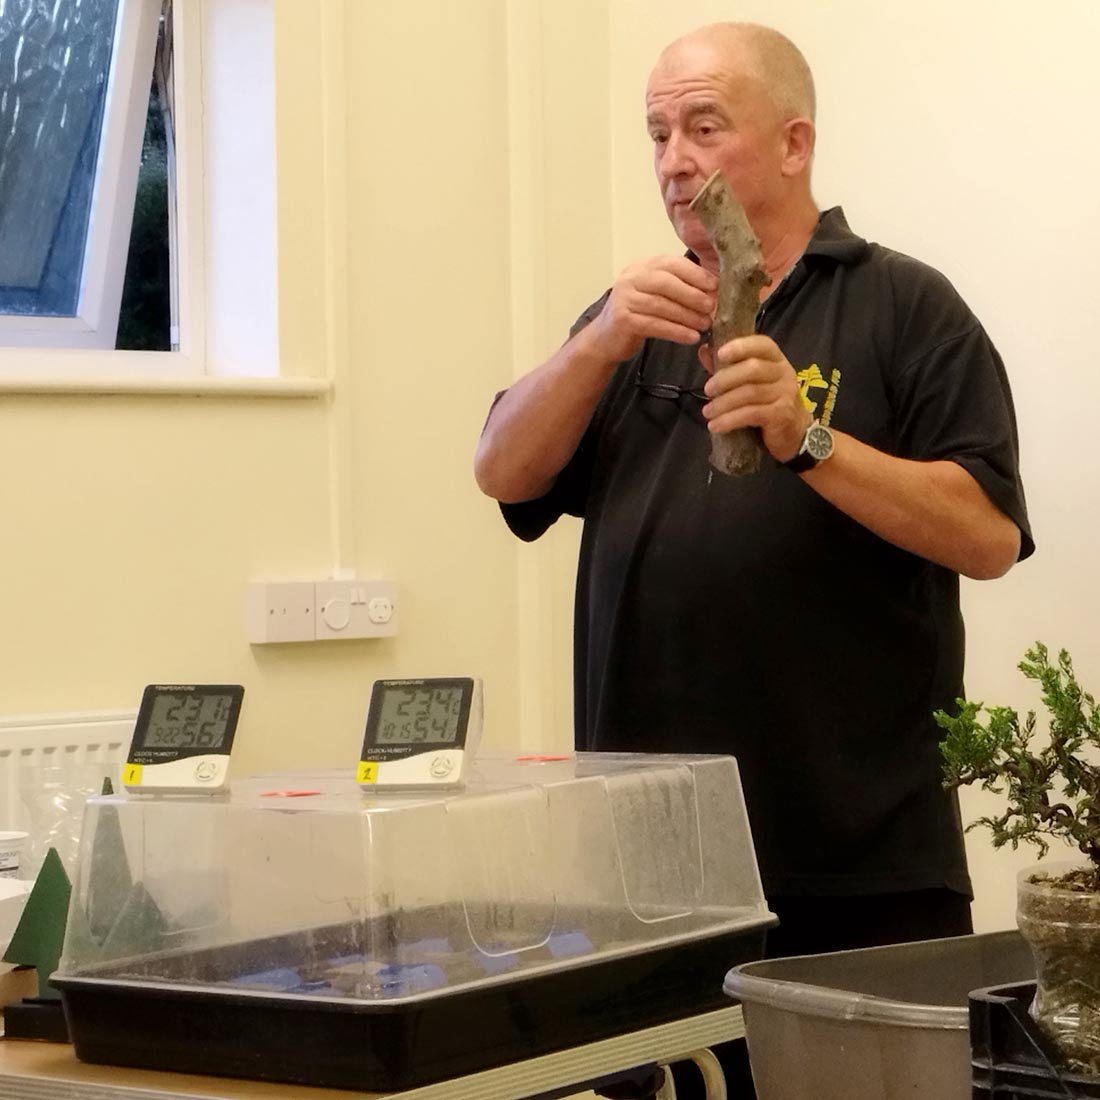
\includegraphics[width=1.0\textwidth]{2025_04/res/humidity_02}
\end{minipage}\qquad
\begin{minipage}[b]{.22\textwidth}
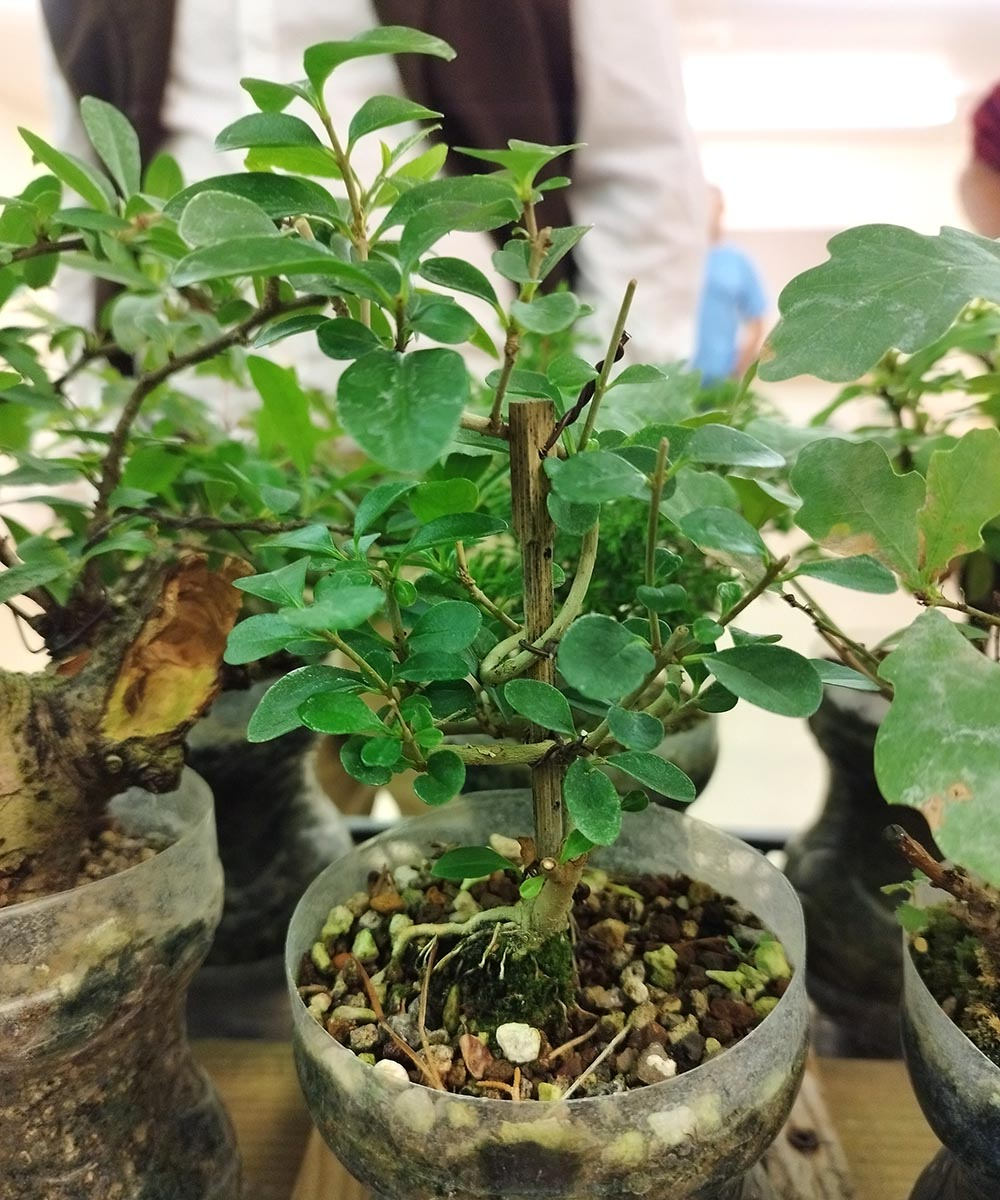
\includegraphics[width=1.0\textwidth]{2025_04/res/humidity_03}
\end{minipage}\qquad
\begin{minipage}[b]{.22\textwidth}
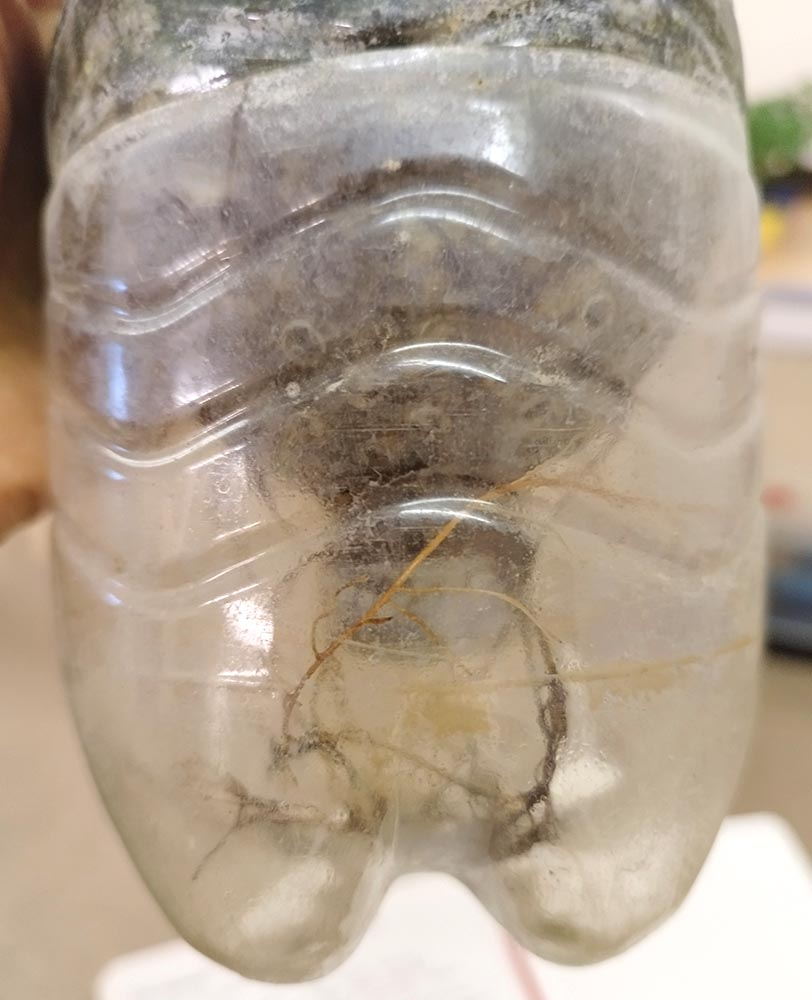
\includegraphics[width=1.0\textwidth]{2025_04/res/humidity_04}
\end{minipage}\qquad
\begin{minipage}[b]{.22\textwidth}
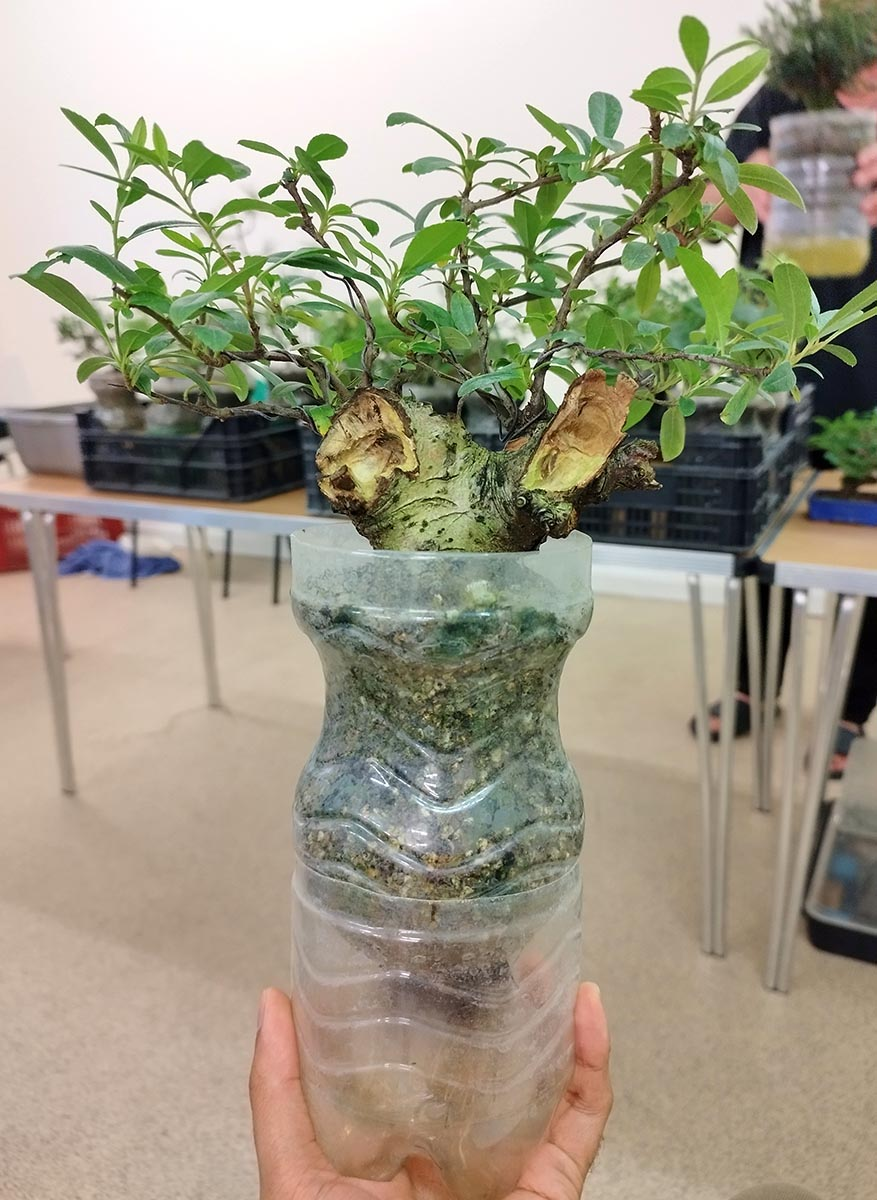
\includegraphics[width=1.0\textwidth]{2025_04/res/humidity_05}
\end{minipage}% \qquad

\medskip
\begin{minipage}[b]{1.0\textwidth}
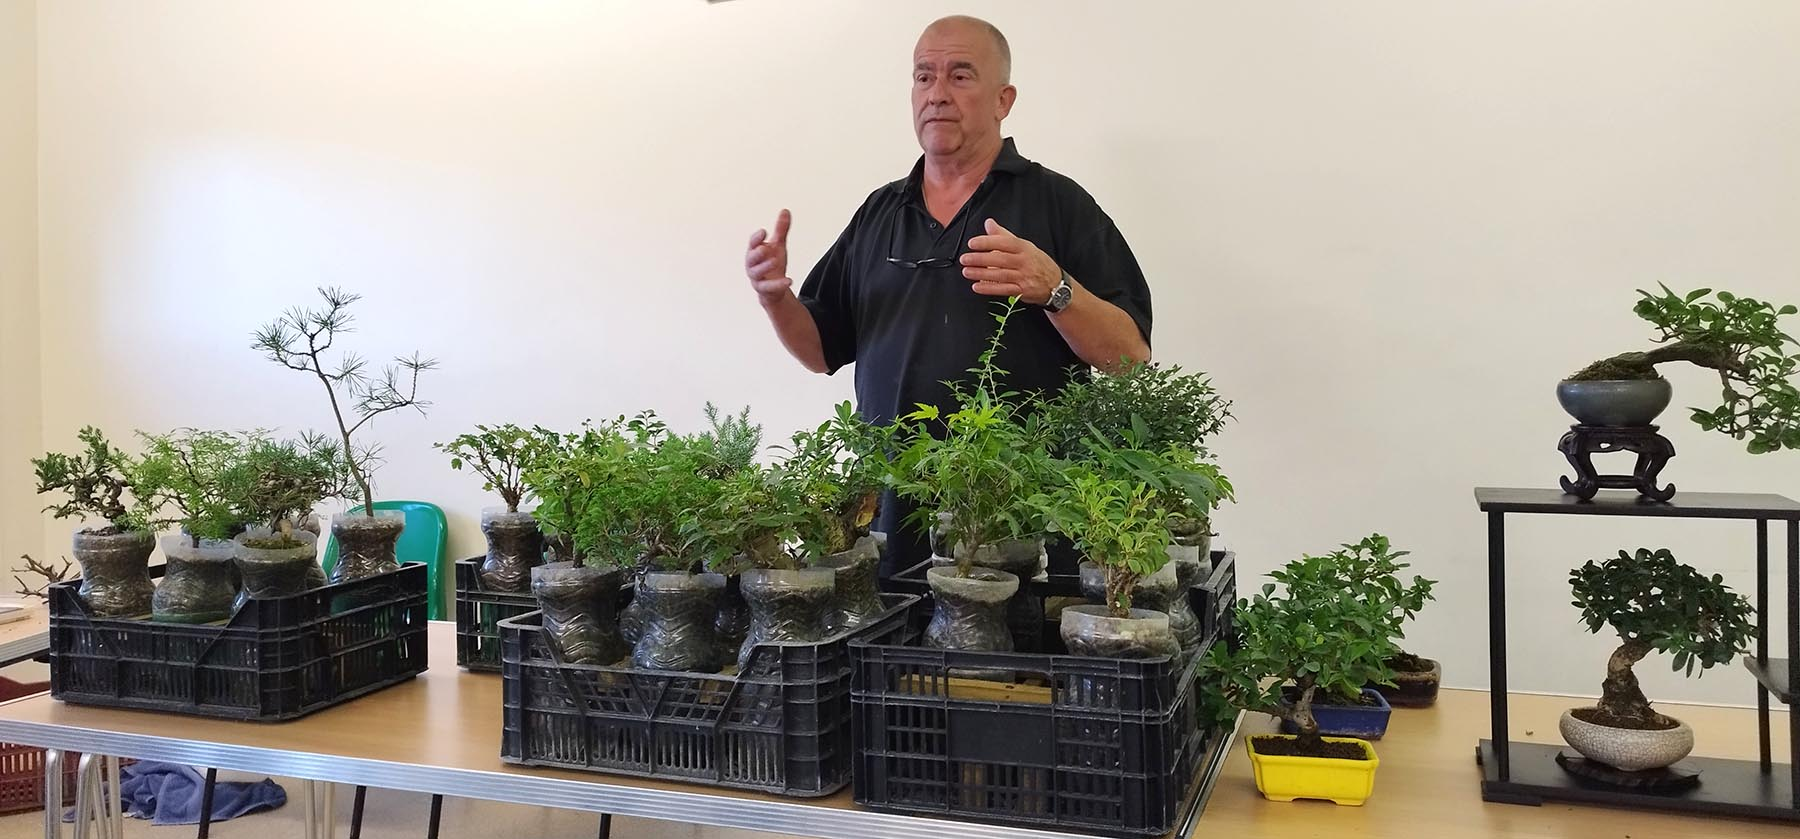
\includegraphics[width=1.0\textwidth]{2025_04/res/humidity_01}
\end{minipage}% \qquad
\centerline{\emph{Mark Moreland explains humidity's role in bonsai growth with his props.}}
\centerline{\emph{(Credit to the Leicestershire Bonsai Club for the photos---completely forgot to take my own!)}}
\end{figure*}

\headline{{\textbf{\Large\sffamily Humidity in Bonsai}}\\
          {\textbf{\large\sffamily By Mark Moreland}}}
\label{2025-04-humidity}
\noindent
Mark Moreland (\href{https://www.ukbonsaiassoc.org}{UK Bonsai Association}) opened his talk by painting a picture of how the bonsai scene in the UK has changed over the years.
Before the 2000s, bonsai was more widespread, with many practitioners and a thriving culture of growing trees locally.
However, in recent decades, the trend has shifted towards importing bonsai from overseas.
While this has made high\--quality trees more accessible, it has also come with its own challenges.

Many areas in the UK that were once sources for wild bonsai material have been stripped, and legal restrictions now prevent tree collection in many places.
As a result, rather than cultivating a robust domestic production system, enthusiasts have found it easier to purchase trees from abroad.
However, importing trees is not as straightforward as one might think, and the cost is not just monetary.

A common assumption is that a larger tree (say, over 50cm tall) should be more expensive than a smaller one (around 20cm), given that it contains more material, requires a bigger pot, and occupies more space.
In reality, both trees may end up costing the same due to the logistical difficulties of transporting smaller bonsai.
Large trees are more resilient to the stresses of shipping, whereas smaller ones are more susceptible to drying out or disease during transit.
The mortality rate of smaller trees in shipping affects pricing, as the costs of lost stock are absorbed into the final price of surviving trees.

To counteract these challenges, Mark focused his talk on developing a local, sustainable method of propagation---one that extends the growing season and reduces dependency on imports.
This method involves using propagation boxes to maintain optimal humidity, creating an environment where cuttings can thrive and root successfully.

\medskip

\topic{The Importance of Humidity}
\noindent
A key theme of Mark's talk was humidity, an often\--overlooked factor in bonsai care.
He explained that when air humidity drops below 50\%, the stomata on leaves close, stopping CO2 absorption, which is crucial for photosynthesis.
This means that in dry conditions, trees essentially stop functioning.
Many people misinterpret this as a tree going into summer dormancy, but in reality, it is struggling due to environmental stress.

Humidity is especially critical for propagation.
Experienced bonsai growers already know that placing an ailing tree in a plastic bag can revive it by creating a humid microclimate.
Mark's propagation method applies this principle to cuttings, ensuring they remain hydrated and are encouraged to root successfully.

\medskip

\begin{figure*}[!p]
\centering
\begin{minipage}[b]{.47\textwidth}
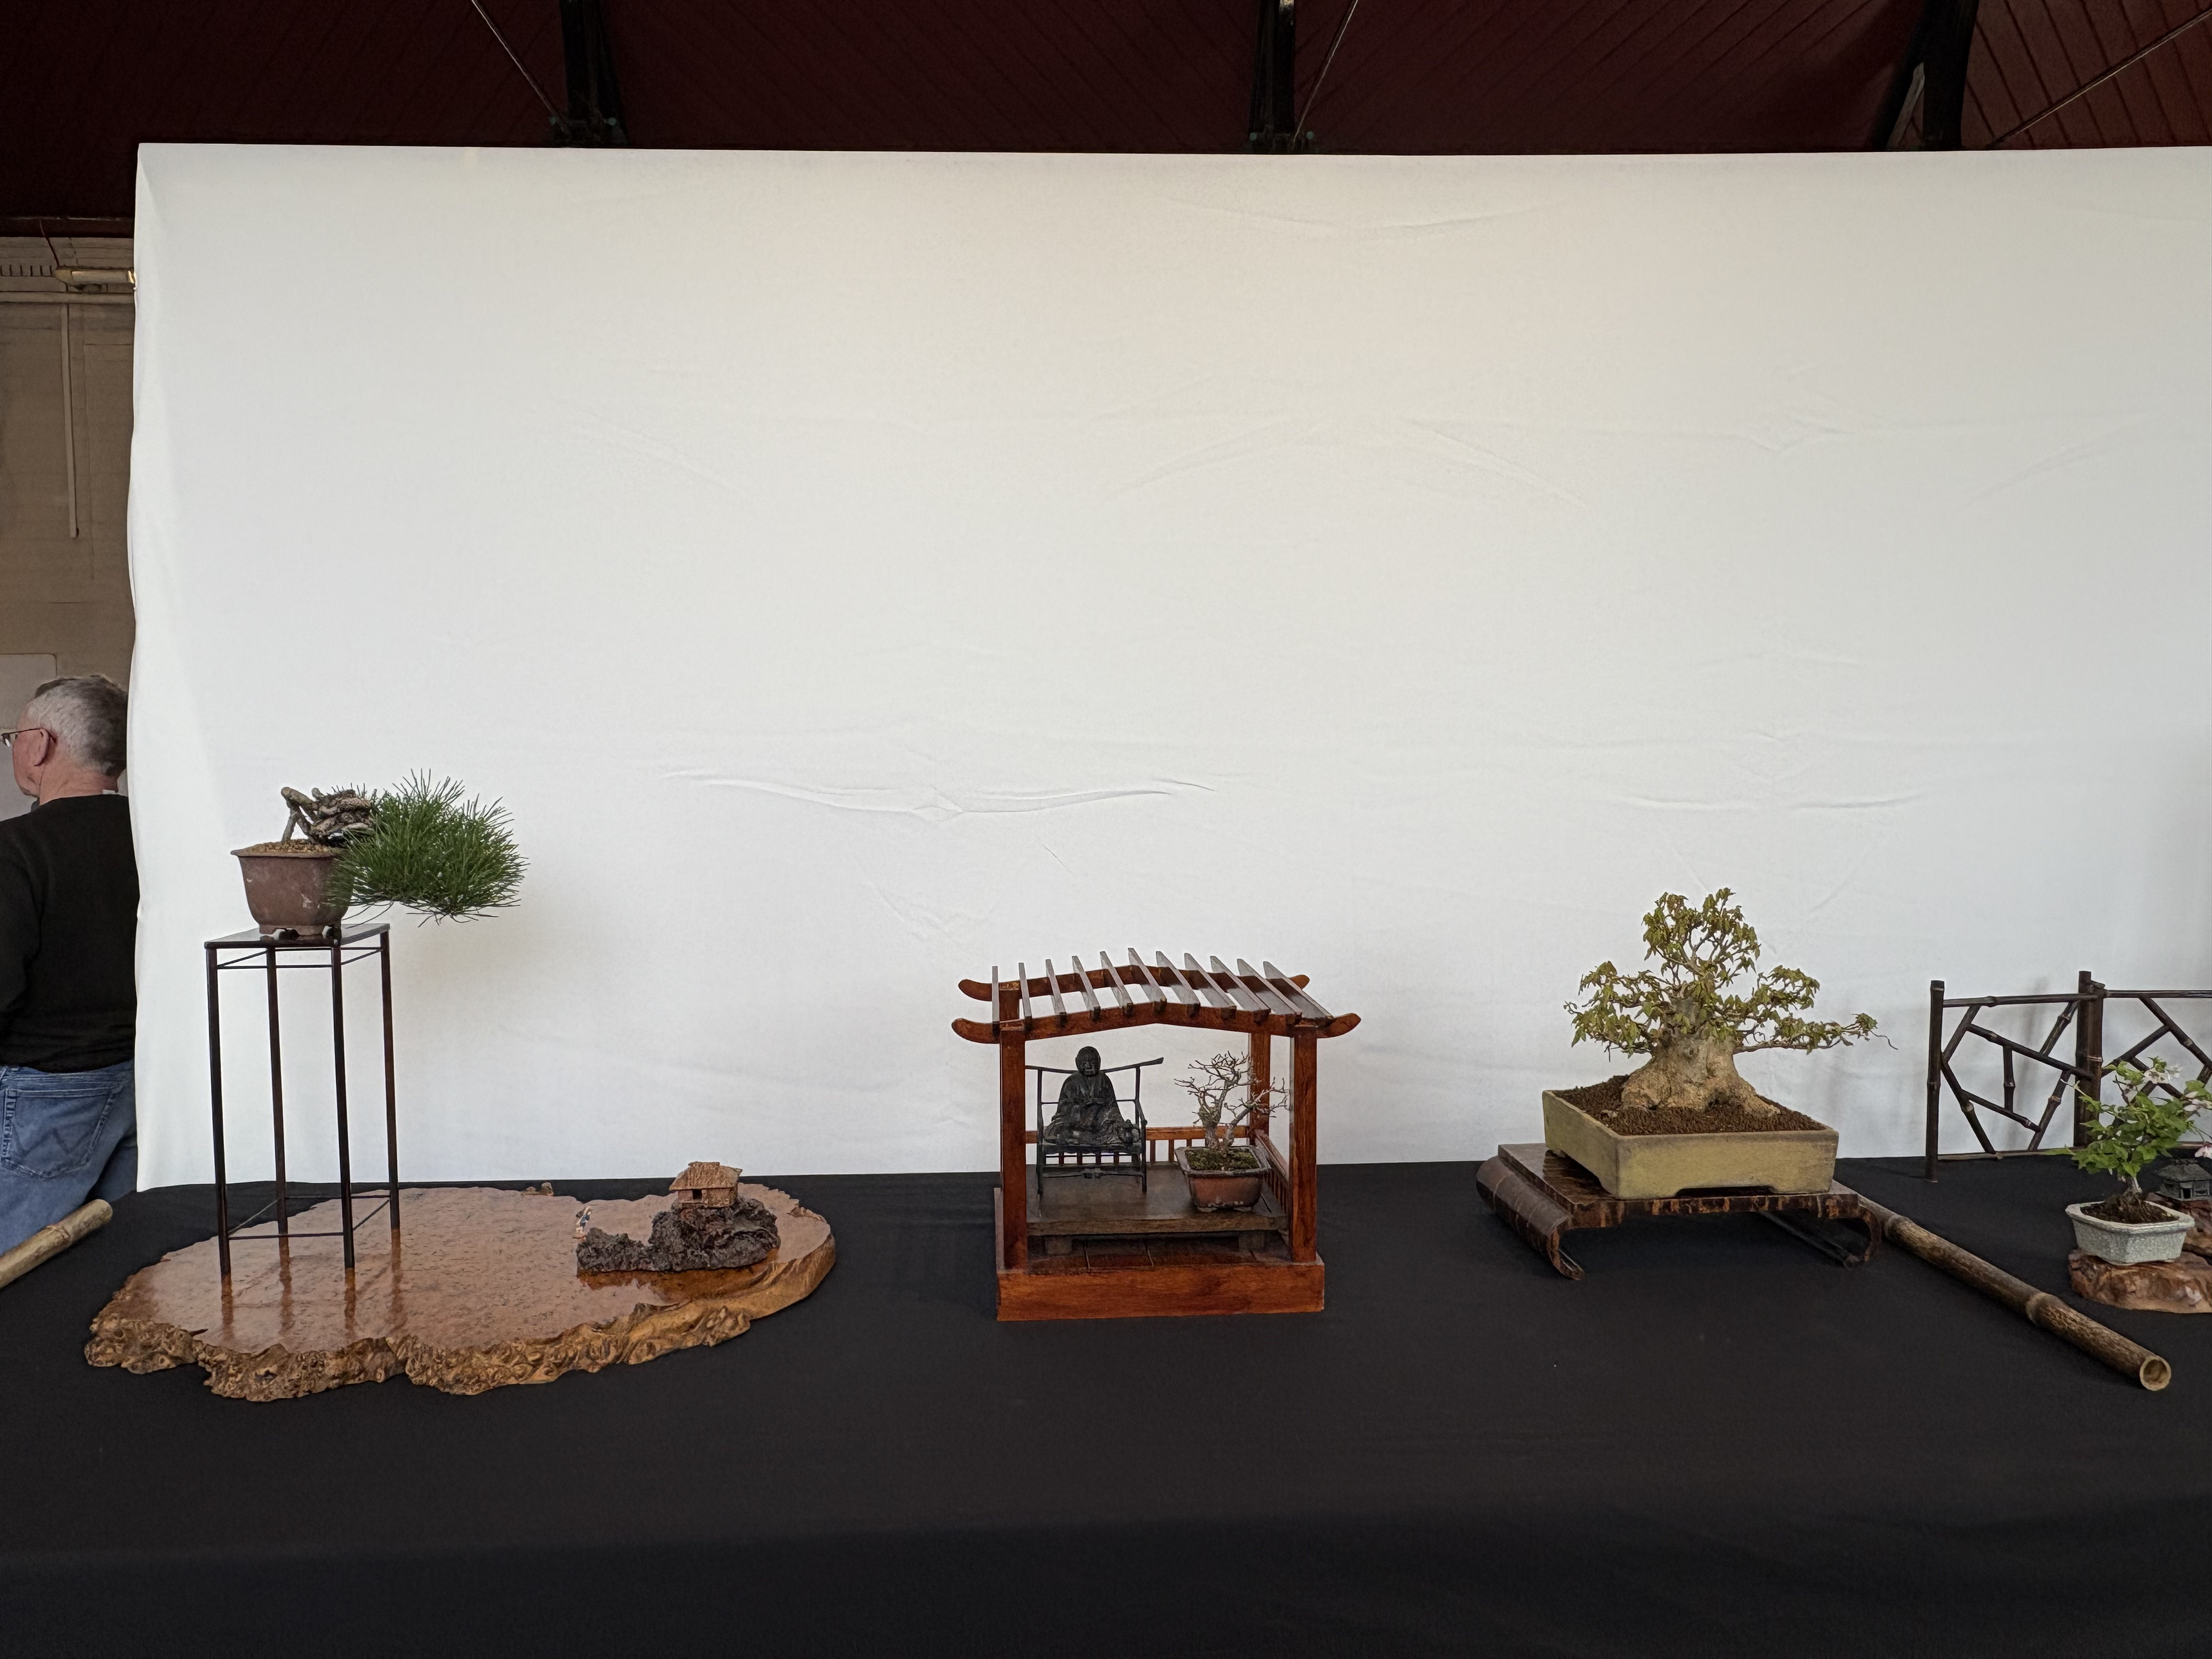
\includegraphics[width=1.0\textwidth]{2025_04/res/display_01}
% \centerline{\emph{David's Hawthorn.}}
\end{minipage}\qquad
\begin{minipage}[b]{.47\textwidth}
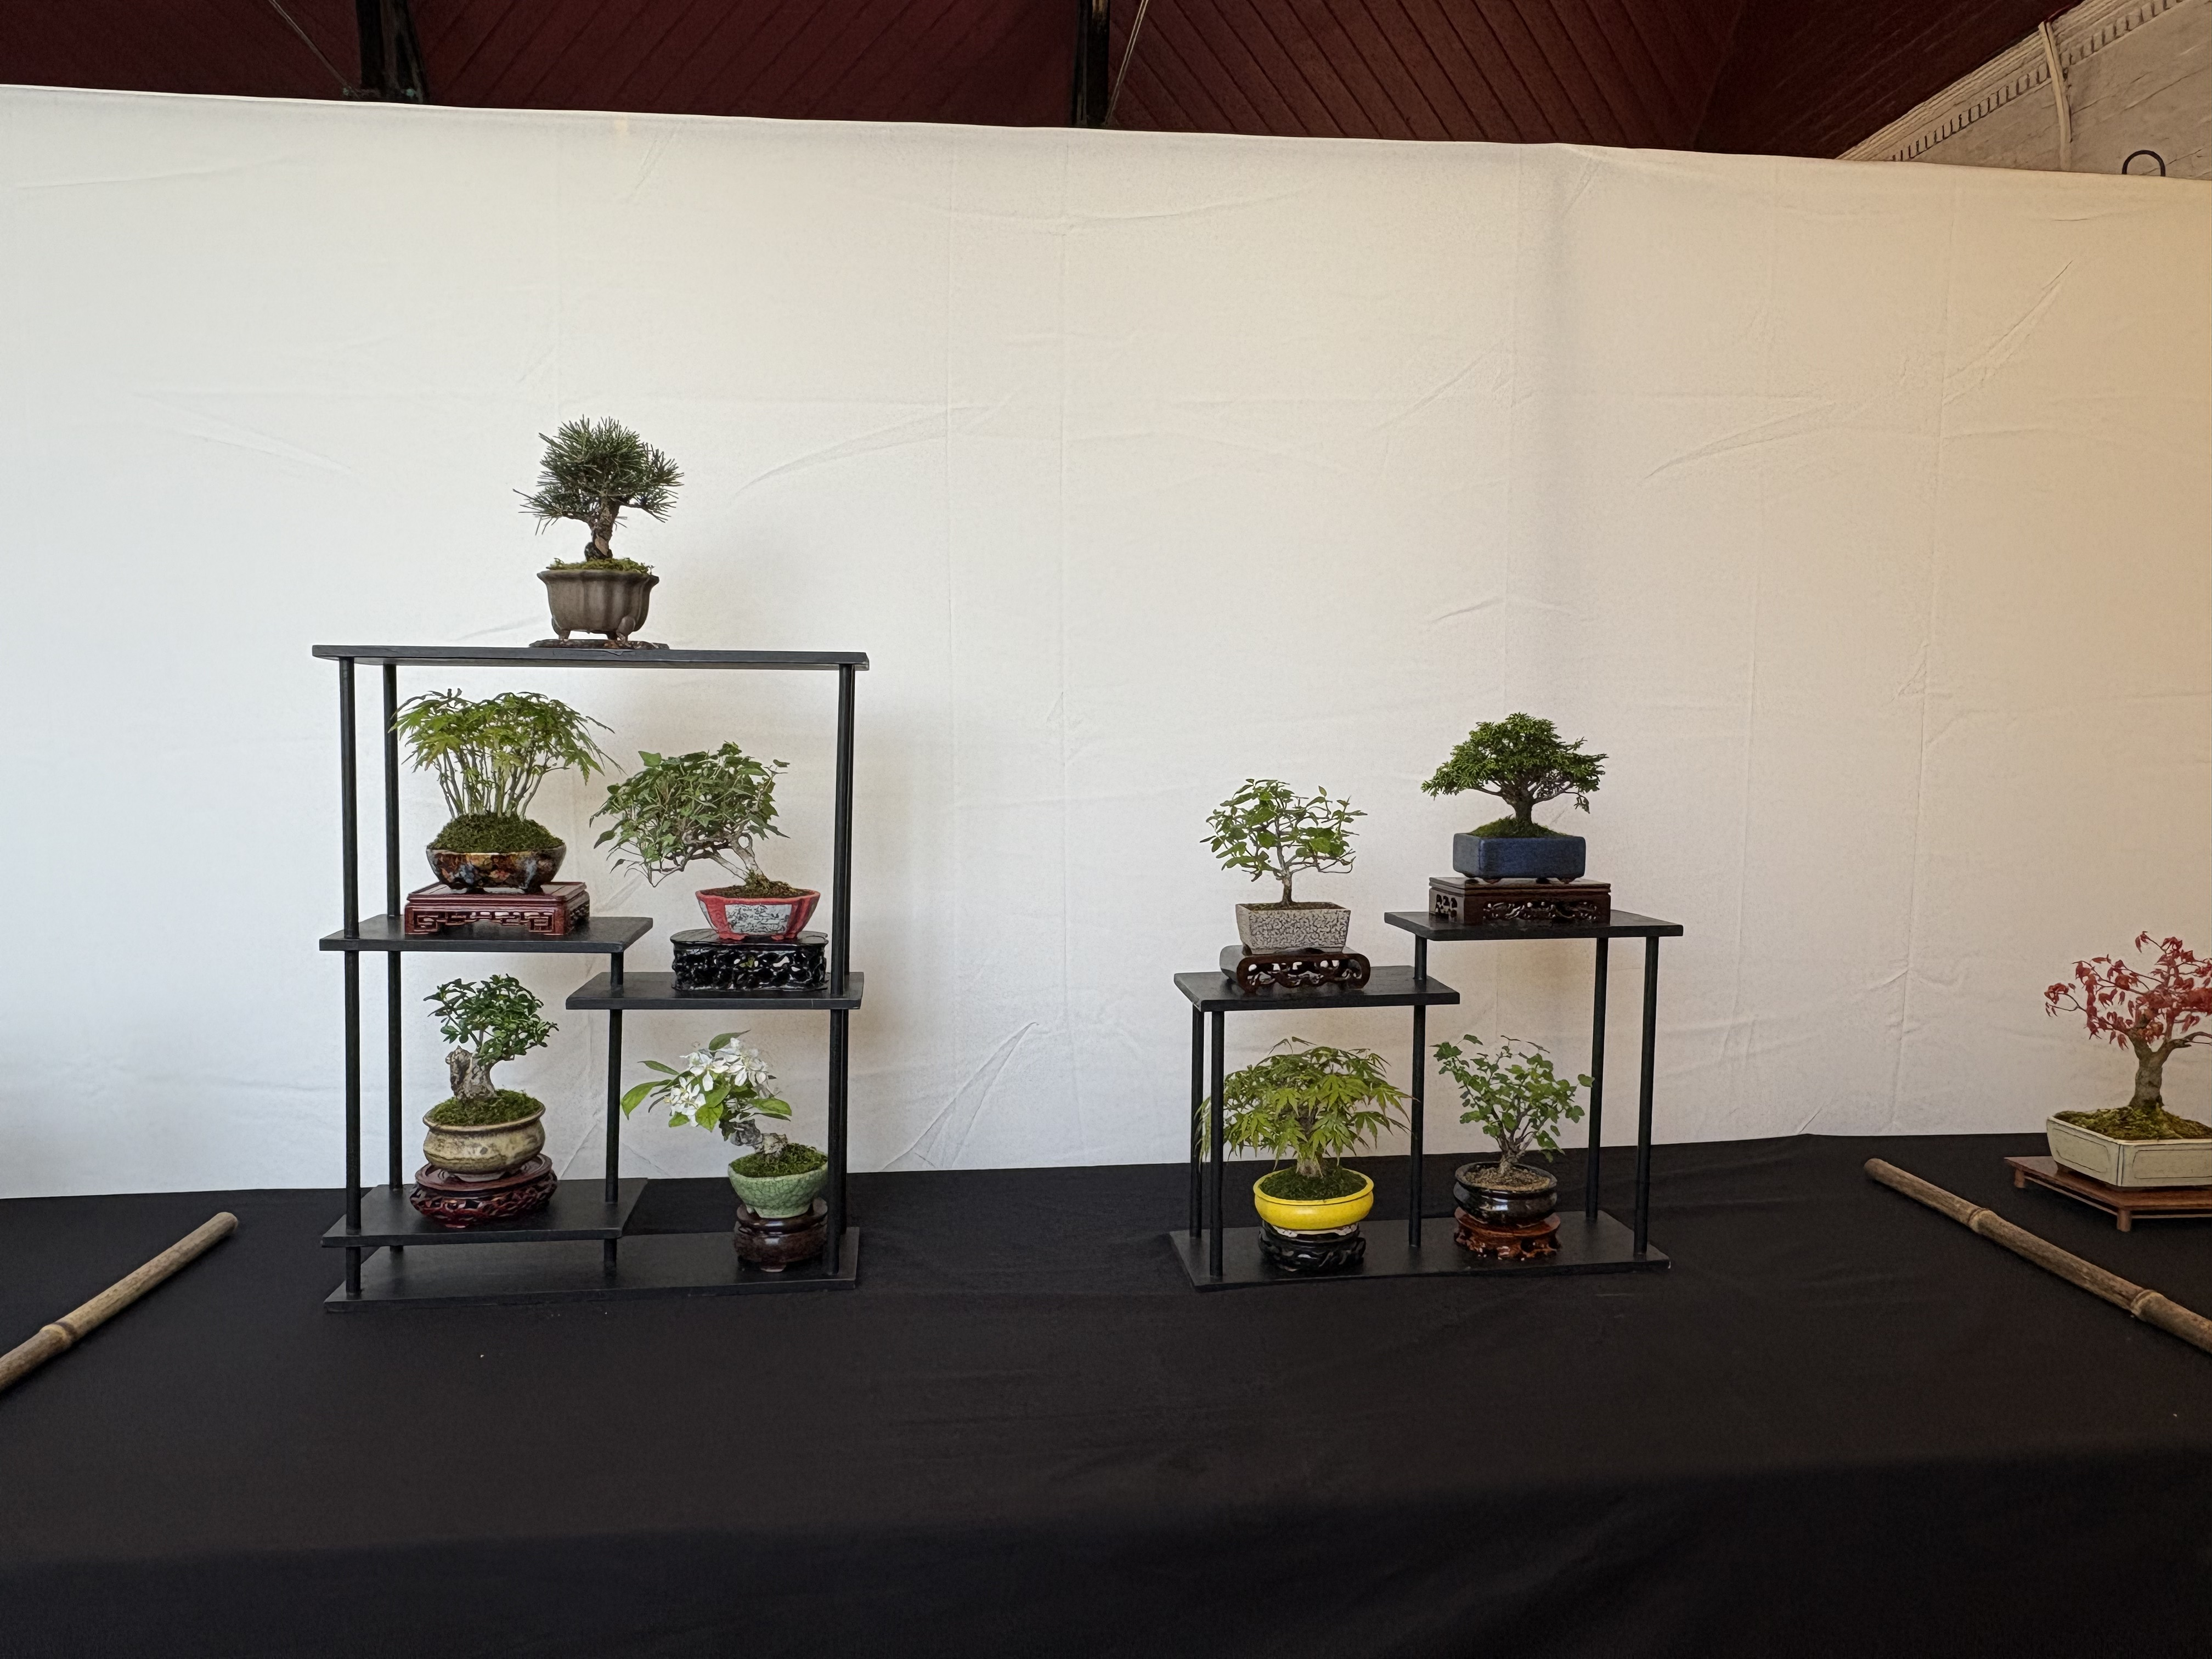
\includegraphics[width=1.0\textwidth]{2025_04/res/display_02}
% \centerline{\emph{Nick's Privet.}}
\end{minipage}
\medskip

\begin{minipage}[b]{.47\textwidth}
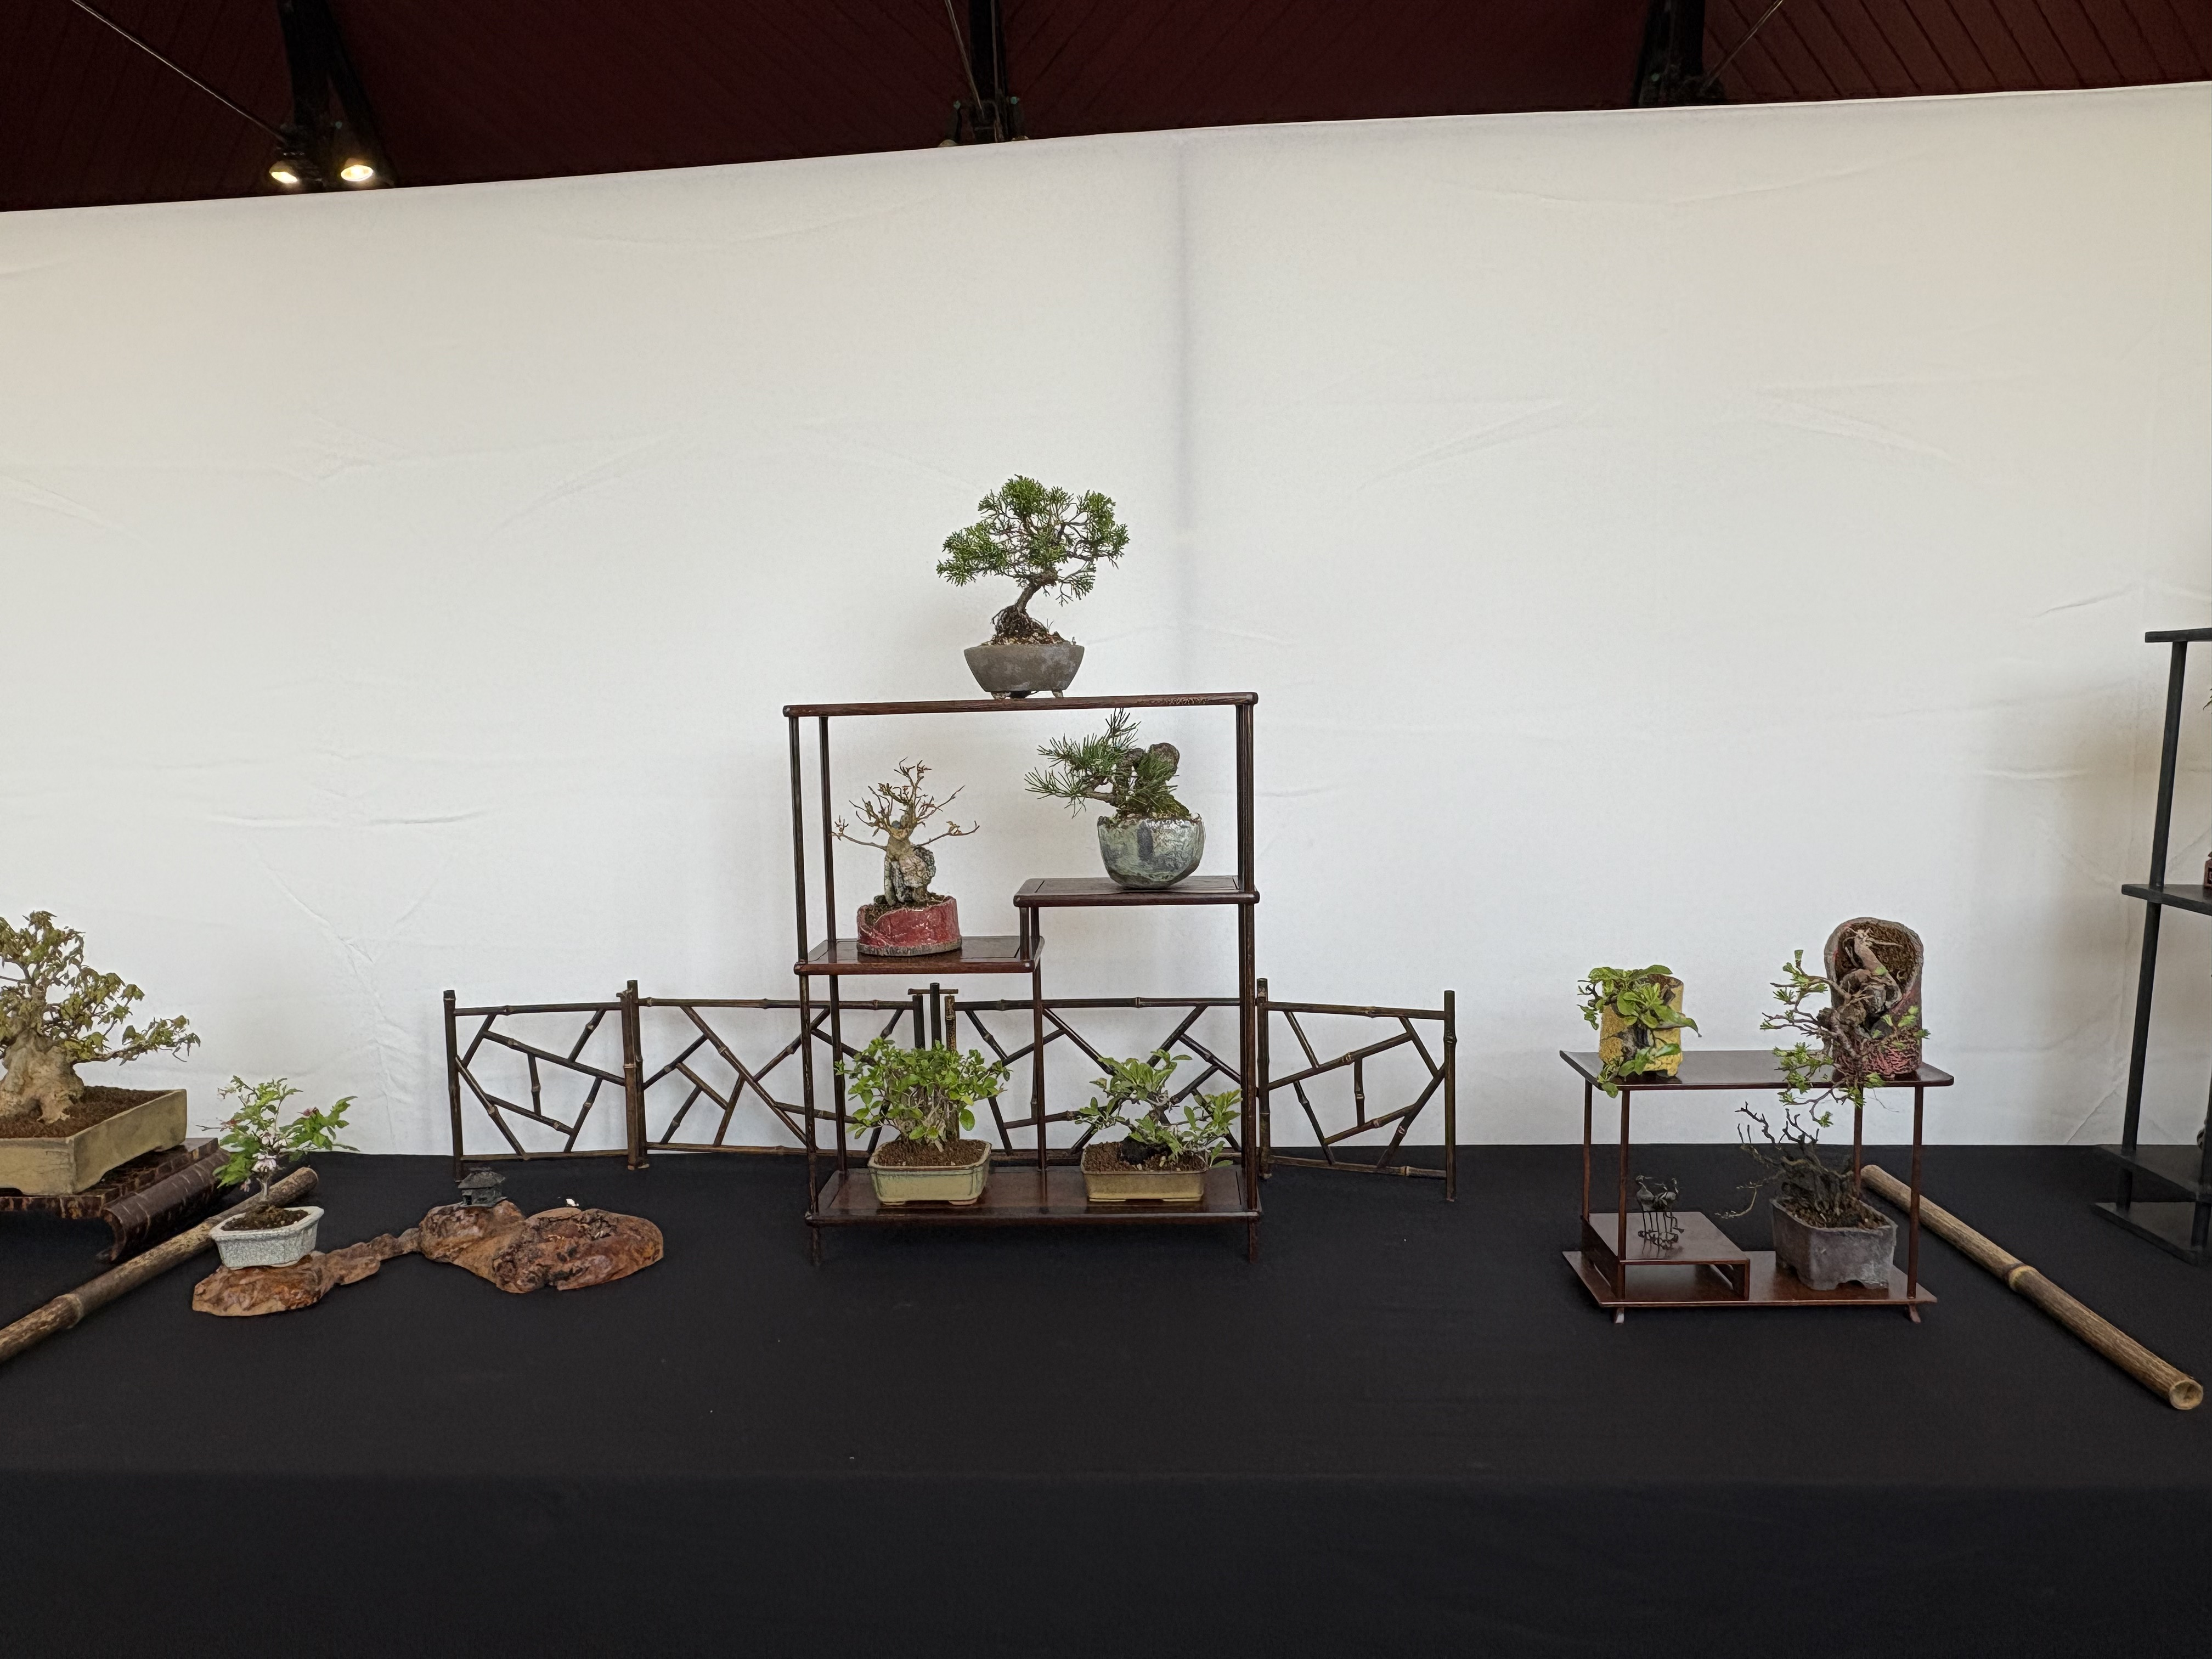
\includegraphics[width=1.0\textwidth]{2025_04/res/display_03}
% \centerline{\emph{Brendan's Yew.}}
\end{minipage}\qquad
\begin{minipage}[b]{.47\textwidth}
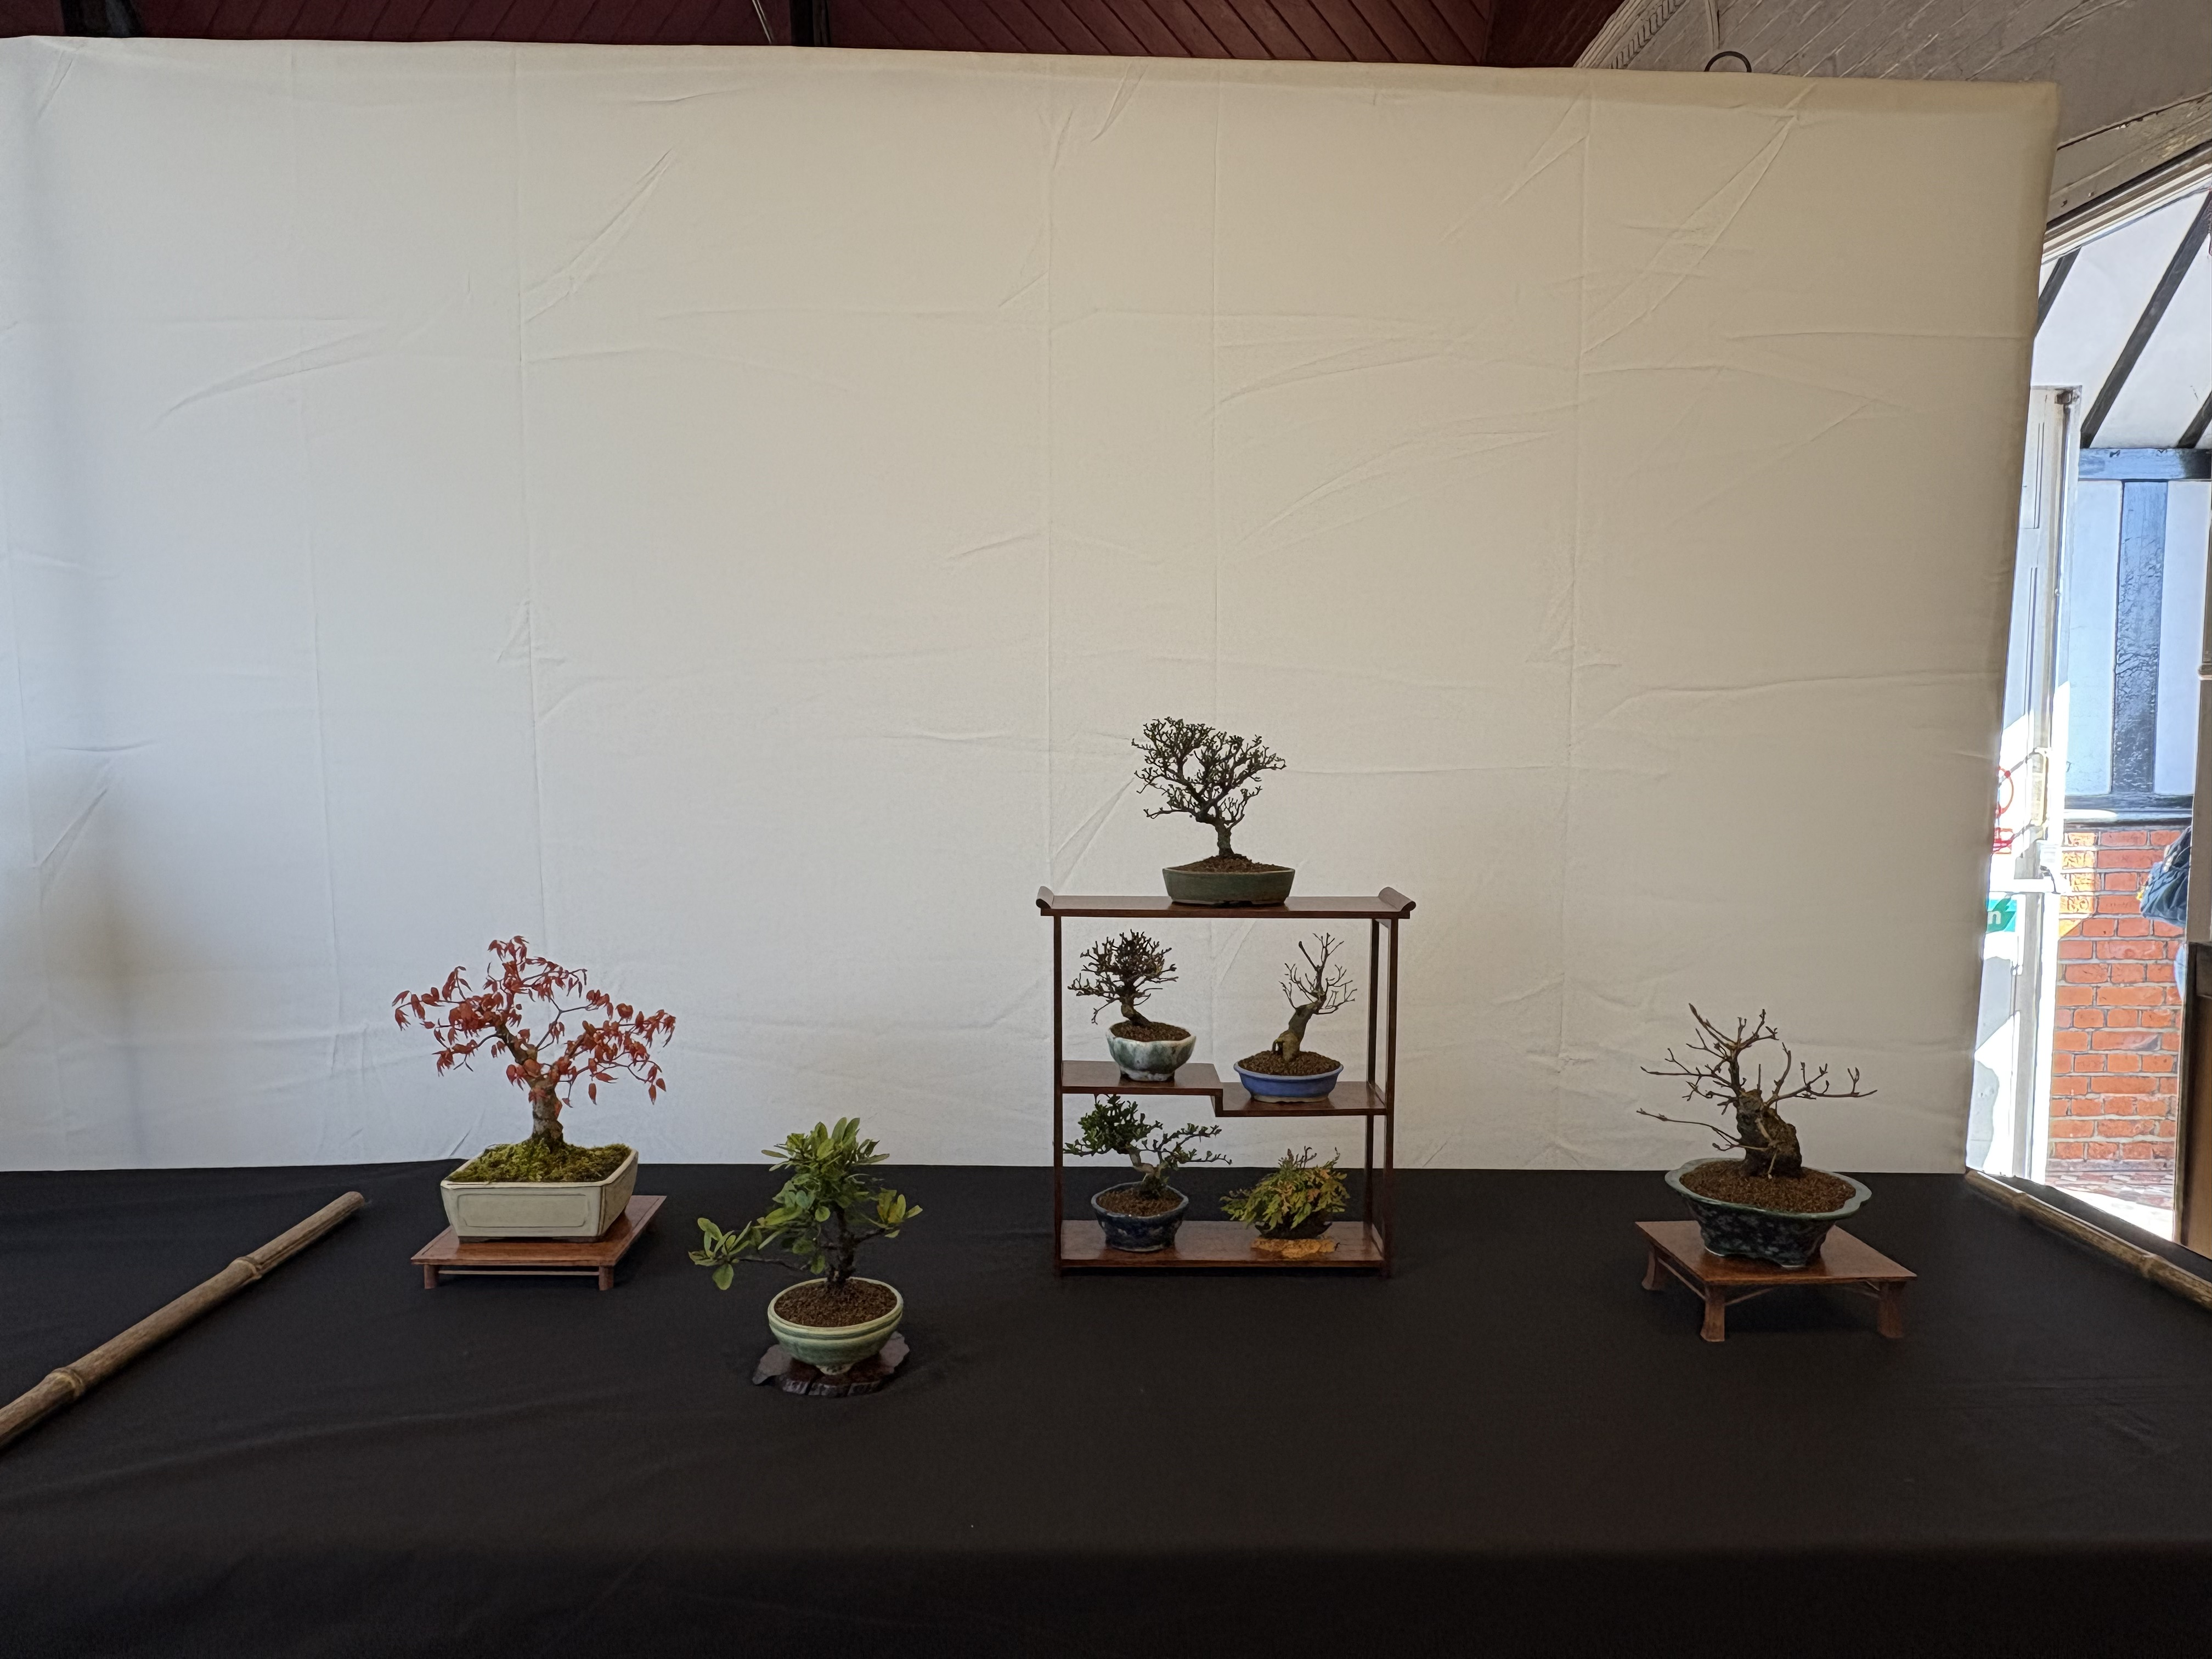
\includegraphics[width=1.0\textwidth]{2025_04/res/display_04}
% \centerline{\emph{Tony's Hawthorn.}}
\end{minipage}
\medskip

\begin{minipage}[b]{.47\textwidth}
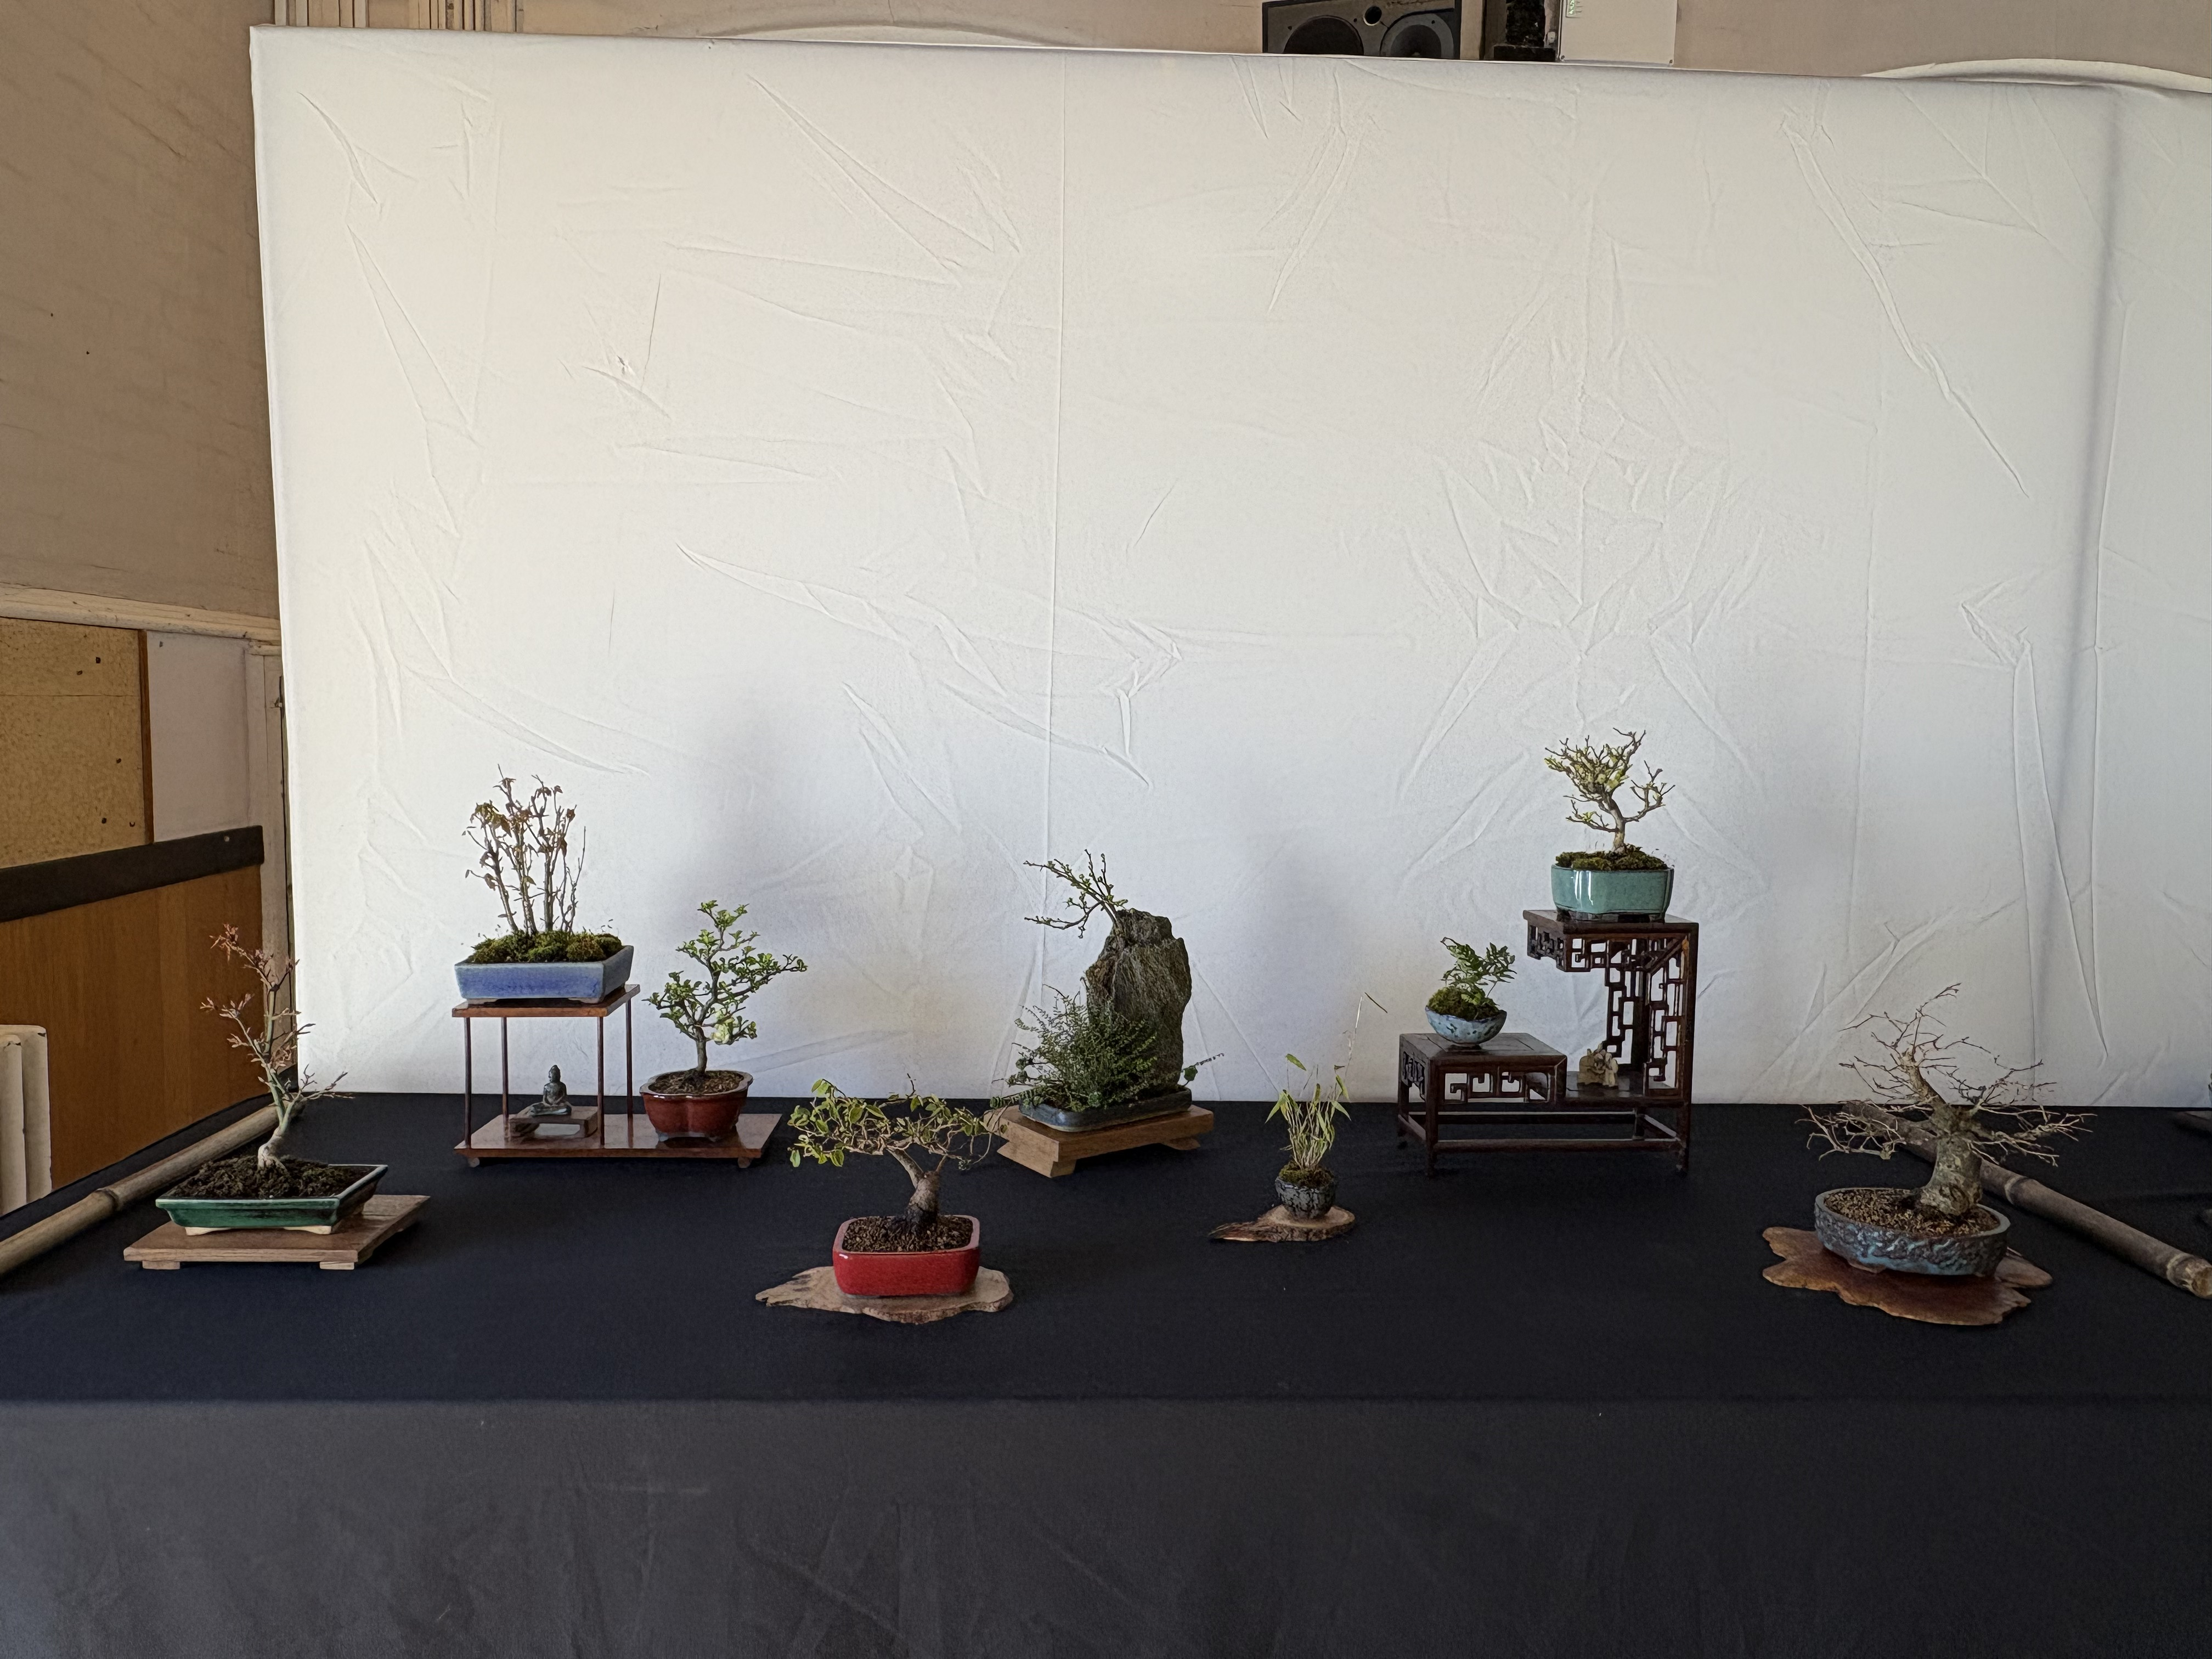
\includegraphics[width=1.0\textwidth]{2025_04/res/display_05}
% \centerline{\emph{Terry's American Sweetgum.}}
\end{minipage}\qquad
\begin{minipage}[b]{.47\textwidth}
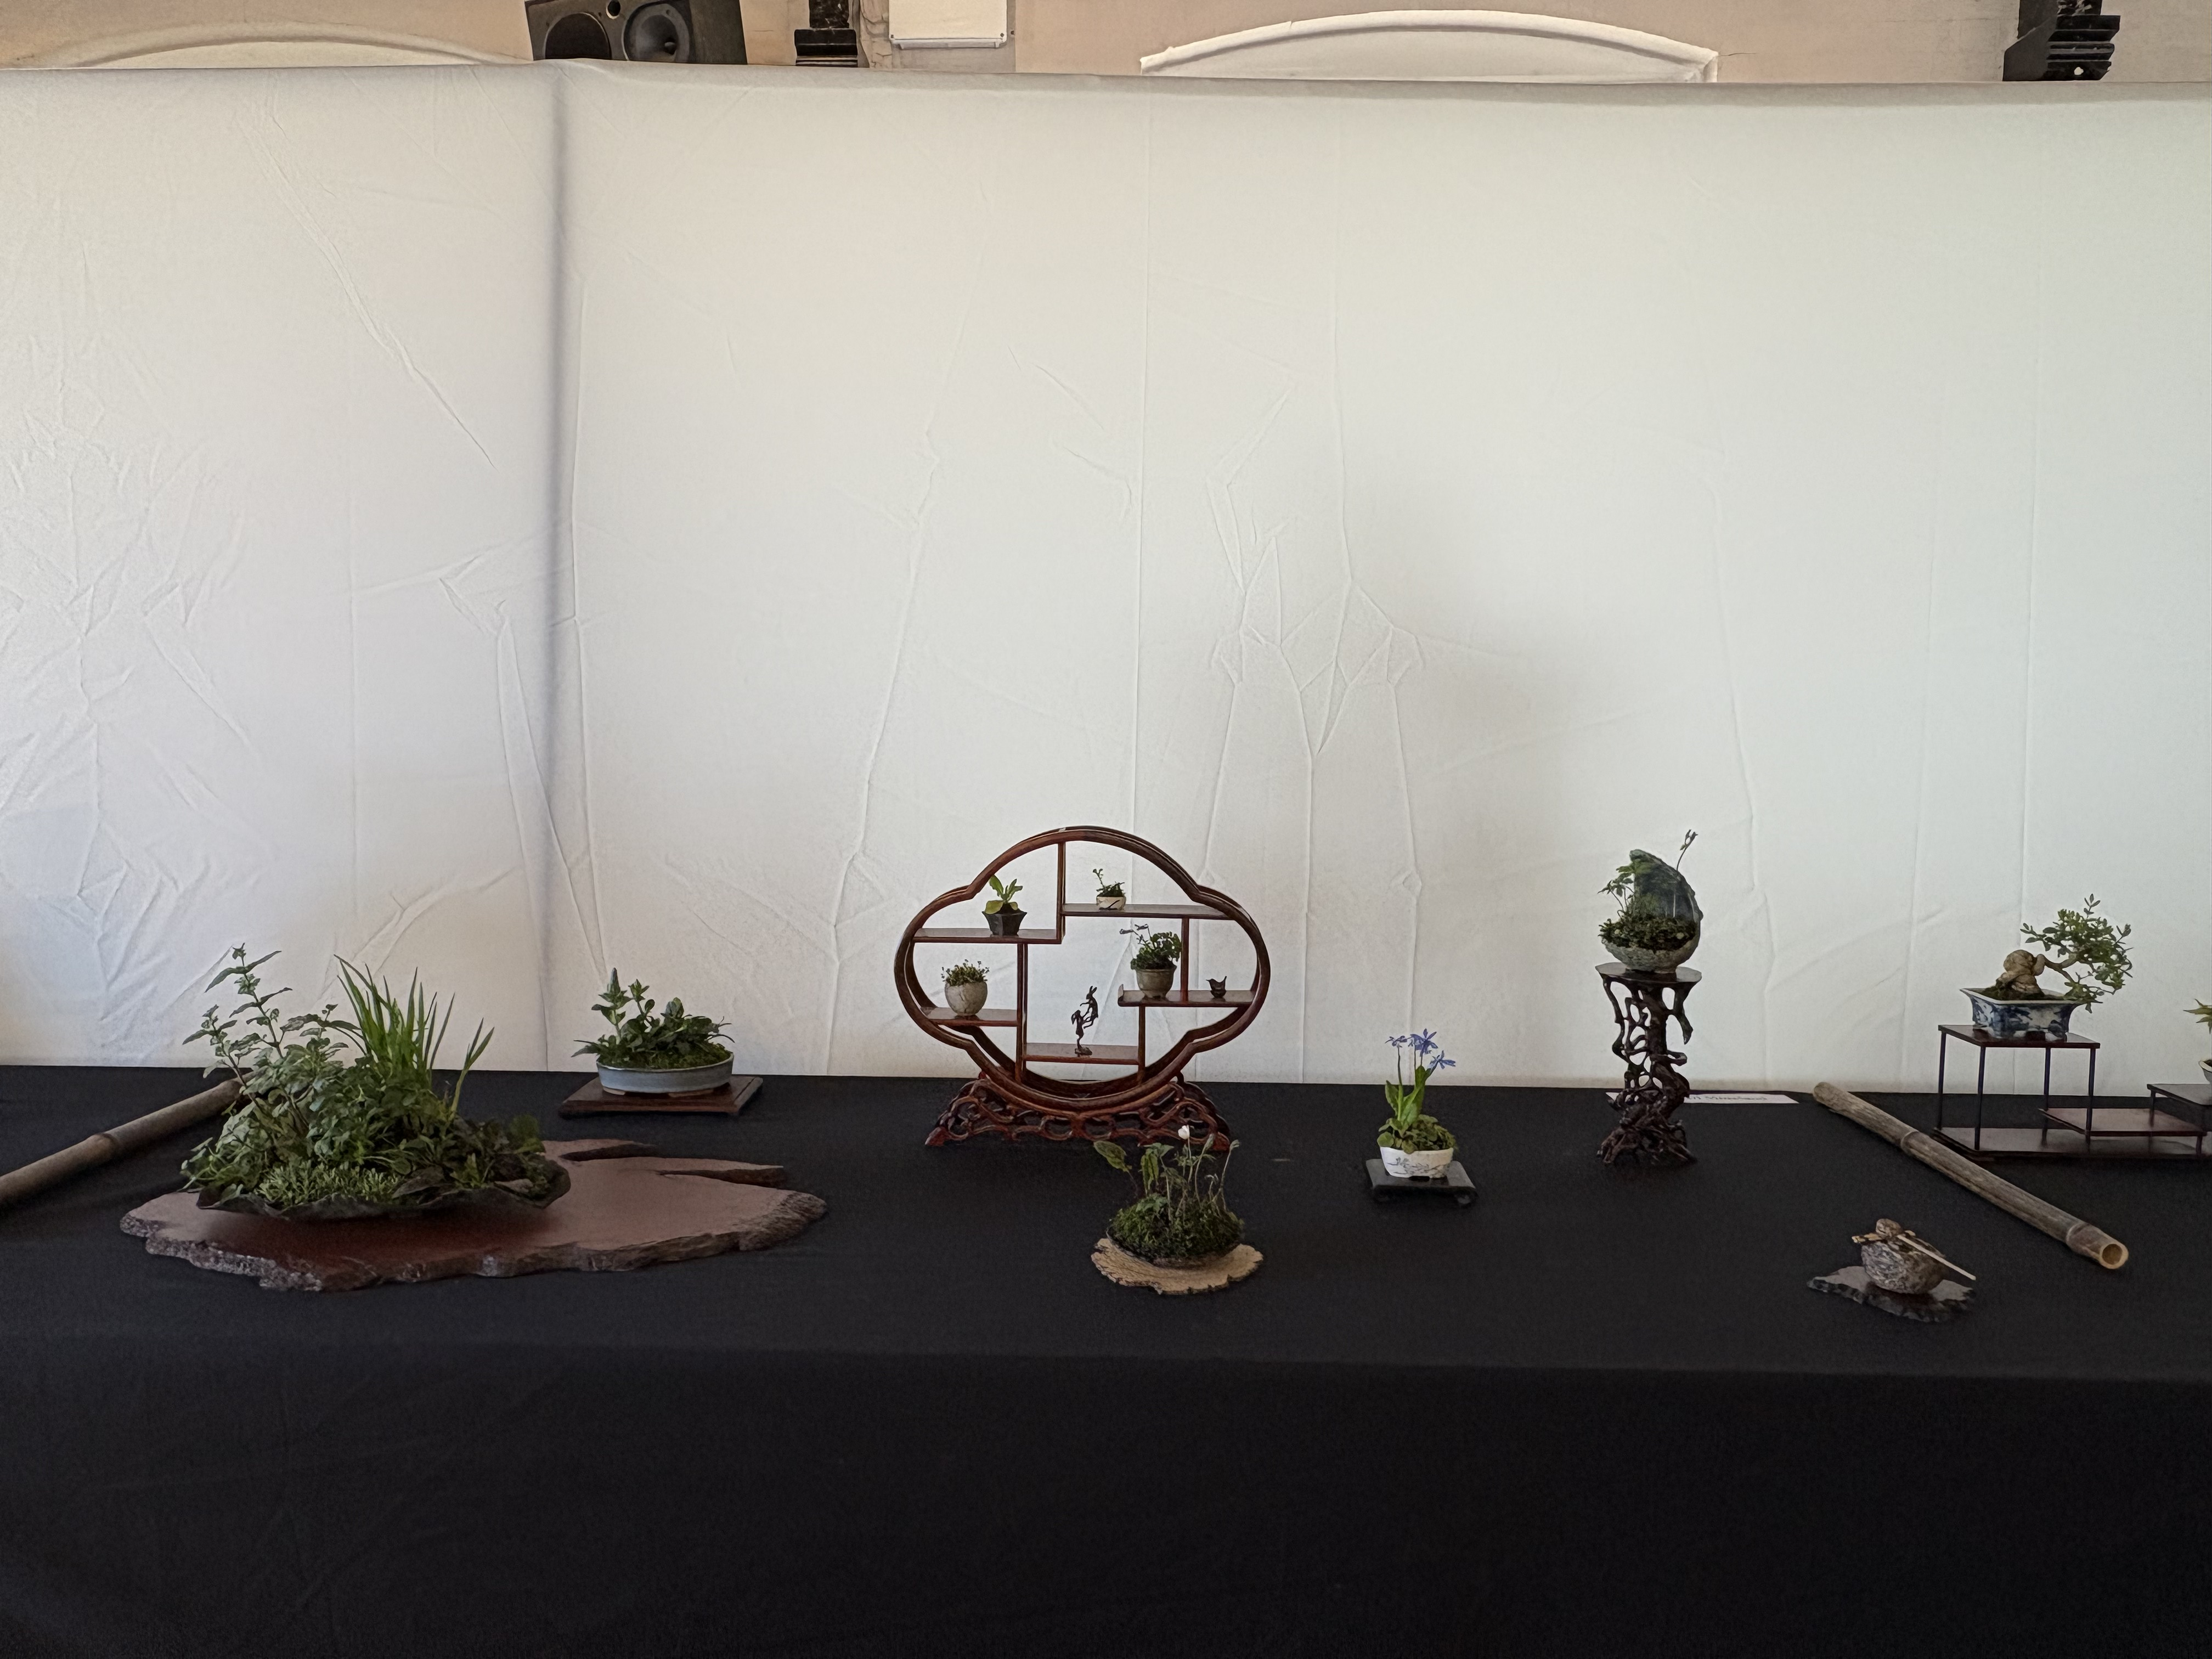
\includegraphics[width=1.0\textwidth]{2025_04/res/display_06}
% \centerline{\emph{Mark's Hawthorn.}}
\end{minipage}
\medskip

% \begin{minipage}[b]{.42\textwidth}
% \includegraphics[width=1.0\textwidth]{2025_01/contest_stefano_benjamina}
% \centerline{\emph{Stefano's Ficus Benjamina.}}
% \end{minipage}

\centerline{%
\emph{The overture of miniature bonsai wonders, gracing Chobham Village Hall.}%
}
\end{figure*}

\topic{Taking and Preparing Cuttings}
\noindent
Mark provided a step\--by\--step guide on how to take and prepare cuttings for propagation:

\begin{itemize}
    \item Select a vigorous shoot from the top of a healthy plant, preferably pencil\--thick, as these have the most stored energy for rooting.

    \item Prevent the cutting from drying out.
    If it needs to be transported, it should be kept moist to maintain its viability.

    \item Strip the lower leaves from the cutting, as this is where roots will develop.

    \item Soak the cutting for a few days in a solution containing a seaweed\--based invigorator, such as Rhizotonic, to stimulate root growth.

    \item Place the cutting into a propagator, where the high humidity will prevent it from drying out and improve the chances of successful rooting.
\end{itemize}

\medskip

\topic{Building a Simple Propagation System}
\noindent
Mark demonstrated a simple, cost\--effective way to build a propagation chamber using a clear plastic drinks bottle.
The process is as follows:

\begin{enumerate}
    \item Cut a clear plastic bottle in half and make holes in the top section and lid using a soldering iron.

    \item Invert the top section and place it inside the bottom half, ensuring it is suspended rather than sitting directly in water.

    \item Use a particulate growing medium, such as pumice, perlite, lava rock, or fired clay, to pot up the cutting.
    This ensures the roots receive adequate air.

    \item Add a small amount of water to the bottom half of the bottle.
    This creates humidity around the roots without waterlogging them.

    \item Capillary matting can be used to help maintain high humidity levels (>80\%).

    \item Use thermometers/hygrometers to monitor the humidity inside and outside the propagator.
\end{enumerate}

This method provides a self\--contained, portable system that maximises rooting success while minimising waste and environmental impact.

\medskip

\topic{Progressing Cuttings and Root Development}
\noindent
Mark has spent several years refining his propagation techniques, experimenting with different trees, substrates, and container setups.
His findings include:

\begin{itemize}
    \item Some species, such as maple, privet, and pyracantha, root easily from smaller cuttings.

    \item Thicker cuttings have been successfully rooted in species like maple and forsythia.

    \item Compared to traditional air layering (which may only yield one new tree), Mark's approach allows a single branch to be divided into multiple cuttings, increasing the chances of success.

    \item The technique is scalable---while Mark primarily uses small propagators, larger storage boxes could be adapted for use, similar to those employed by houseplant growers.
\end{itemize}

\medskip

\topic{Practical Tips for Successful Propagation}
\noindent
Mark shared several tips to improve propagation success and make the process more efficient:

\begin{itemize}
    \item \textbf{Location:} The propagator should be kept in an unheated greenhouse or a protected outdoor space to shield it from wind, pests, and temperature extremes.

    \item \textbf{Managing humidity:} When humidity levels exceed 95\%, prop the lid open slightly to allow airflow and prevent fungal issues.
    Mark typically keeps the lid closed during hot, dry days and opens it at night when conditions are cooler.

    \item \textbf{Watering:} To water the cuttings, lift the top section out, refresh the water in the bottom, and dunk the top section twice in a nutrient solution.
    This prevents overwatering while ensuring adequate hydration.

    \item \textbf{Root trimming:} If roots grow into the water, they can still absorb oxygen, but occasional trimming encourages a denser, more compact root system ideal for bonsai.

    \item \textbf{Off\--season repotting:} Because of the high humidity, bonsai cuttings can be repotted outside the usual spring window.
    Trees remain stable and continue growing as long as conditions inside the propagator are maintained.

    \item \textbf{Seasonal results:} Mark found that maple cuttings taken in March rooted by June, and those taken in July rooted by October.
    This effectively extends the growing season, allowing for greater flexibility.

    \item \textbf{Cold weather considerations:} If the water in the bottom freezes during winter, the cuttings remain unharmed as the roots are above the ice, with air still circulating around them.
\end{itemize}

\medskip

\begin{figure*}[!b]
\centering
\begin{minipage}[b]{.47\textwidth}
\includegraphics[width=1.0\textwidth]{2025_04/res/pots_01}
\end{minipage}\qquad
\begin{minipage}[b]{.47\textwidth}
\includegraphics[width=1.0\textwidth]{2025_04/res/pots_02}
\end{minipage}
\medskip 

\begin{minipage}[b]{.30\textwidth}
\includegraphics[angle=270,origin=c,width=1.0\textwidth]{2025_04/res/pots_03}
\end{minipage}\qquad
\begin{minipage}[b]{.30\textwidth}
\includegraphics[angle=270,origin=c,width=1.0\textwidth]{2025_04/res/pots_04}
\end{minipage}\qquad
\begin{minipage}[b]{.30\textwidth}
\includegraphics[angle=270,origin=c,width=1.0\textwidth]{2025_04/res/pots_05}
\end{minipage}
\medskip 

\centerline{%
\emph{Alex Rudd's gorgeous mame bonsai pots, showcased in his talk.}}
\end{figure*}

\topic{Final Thoughts: Making Bonsai More Accessible}
\noindent
Mark concluded his talk by emphasising the benefits of propagating bonsai locally rather than relying on imports.
His method allows for the production of a greater number of trees, which is particularly valuable for bonsai exhibitions where diversity in species and styles is desirable.
The portability of the propagators also makes it easy to transport and care for trees, even in less\--than\--ideal conditions.

Anecdotally, he shared that before a show, he keeps a stack of propagators in his car for a week, and rather than suffering, the trees actually thrive---putting out fresh green growth despite the confinement.
This underscores the effectiveness of the system in creating a stable environment for bonsai development.

For anyone looking to grow their own bonsai from cuttings, Mark's approach offers a simple, sustainable, and highly effective solution.
By combining practical knowledge with a deep understanding of plant physiology, he has provided an accessible method that can help reinvigorate the UK's bonsai community and ensure the continued growth of this beautiful art form.

\begin{center}
    $\cdots$
\end{center}
% \noindent
\textit{Unfortunately, I missed the first few minutes of the talk, so I’ve done my best to piece together the missing part using notes from a similar talk last year, as recorded by the Leicestershire Bonsai Club at \href{https://leicsbonsaiclub.wordpress.com/2024/09/03/mark-moreland-visit-03-09-24/}{this link}.}

\closearticle
\columnbreak
